\chapter{Change of Variables}

Let's say that I'm making ice spheres, and I tell you that the radius of the ice spheres is normally distributed with a mean
of 0.7 cm and a standard deviation of 0.08 cm.   Then you can draw the probability distribution and cumulative distribution for that:

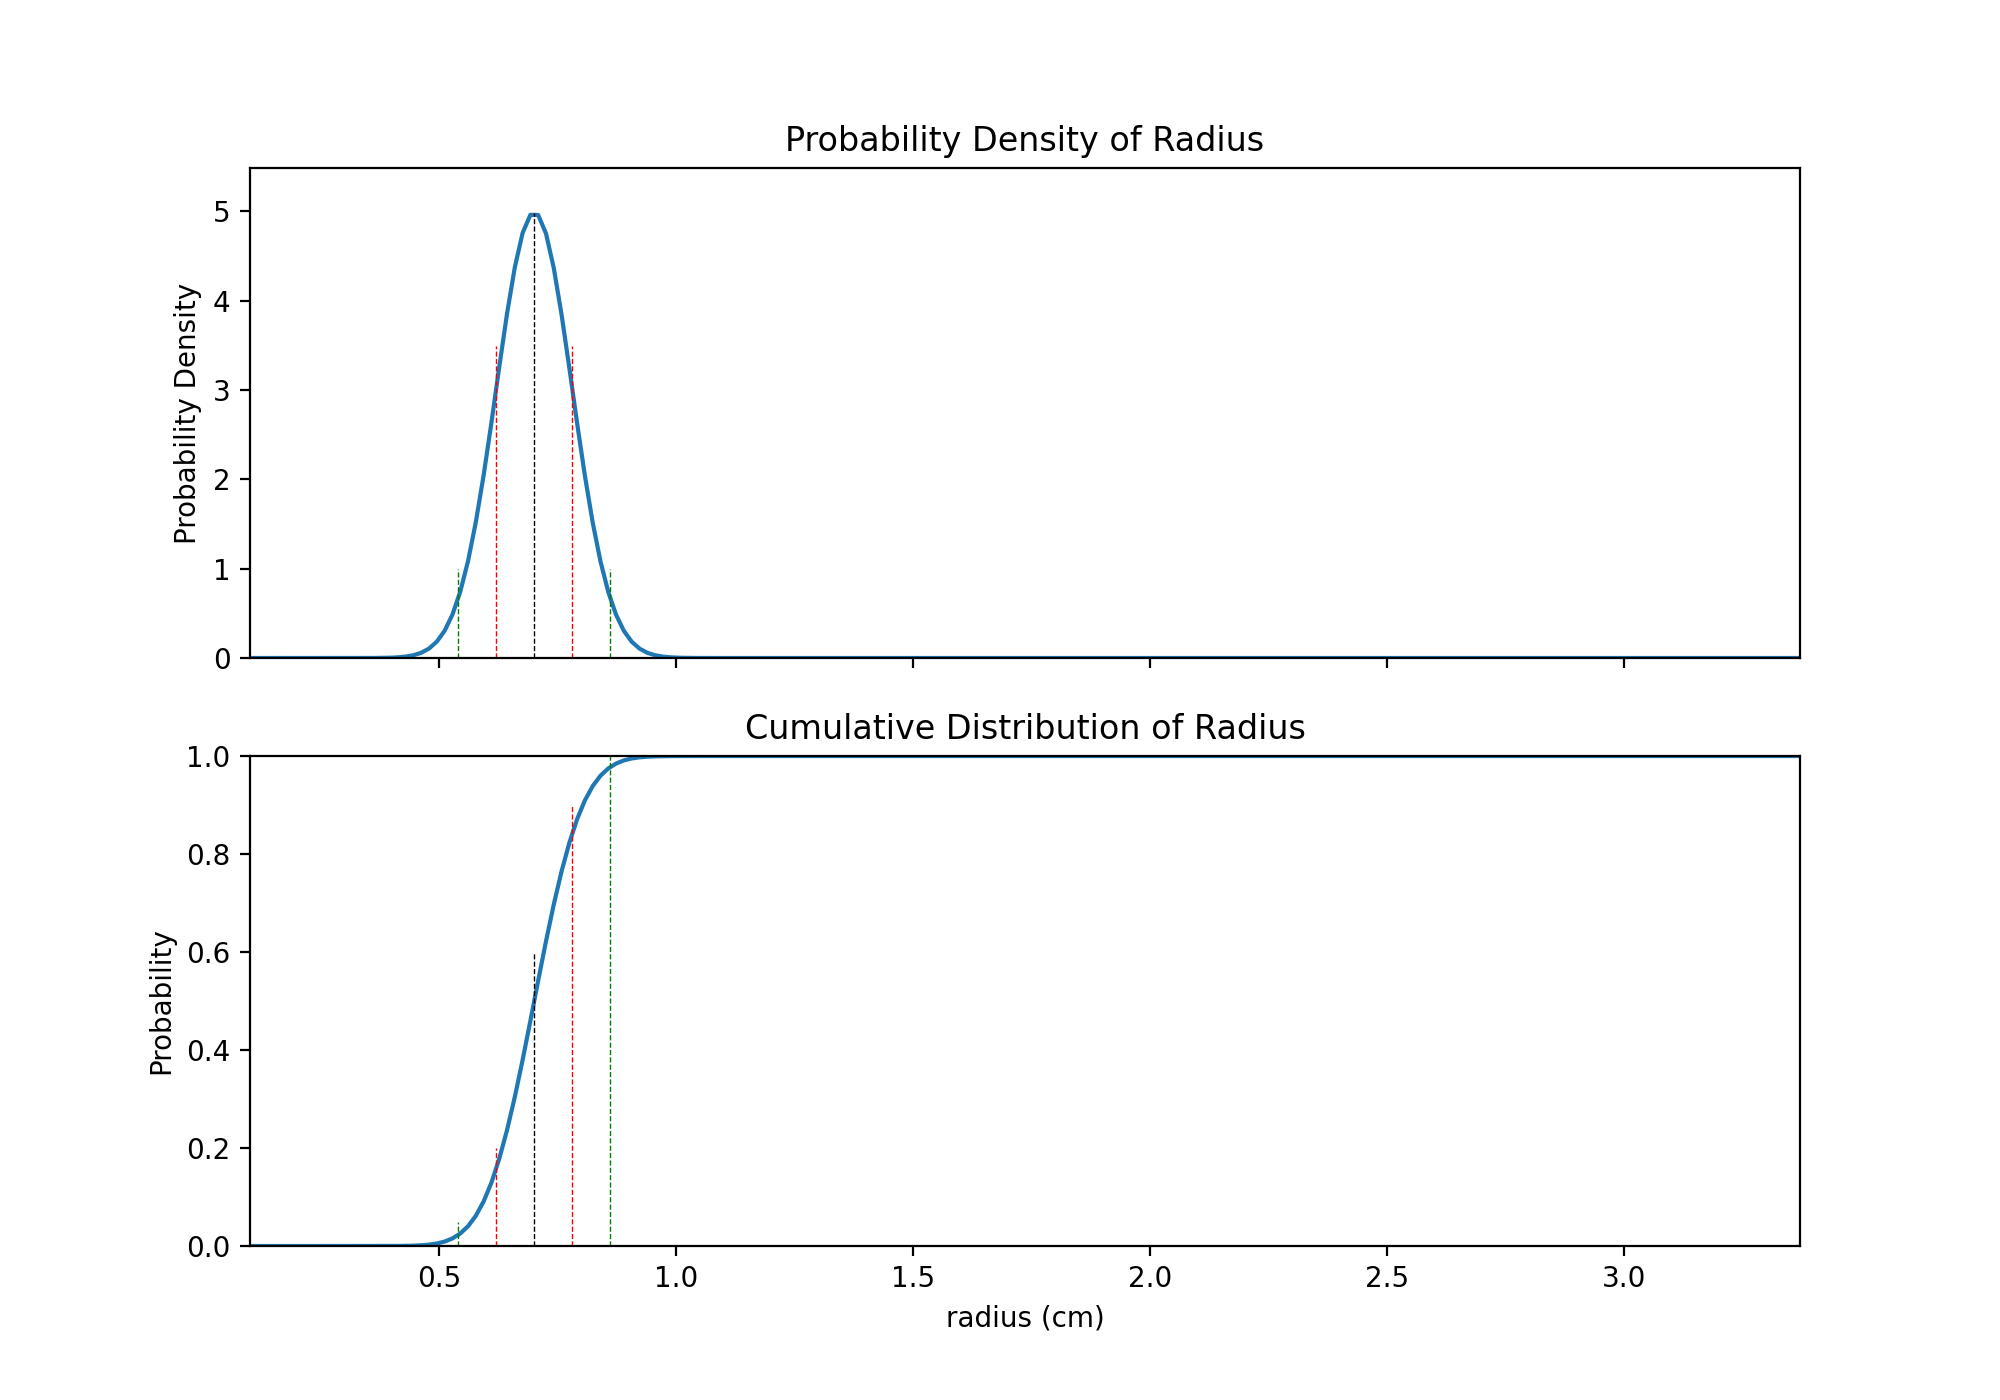
\includegraphics[width=0.8\textwidth]{before.png}

This includes lines indicating the mean and two standard deviations on each side.

Now,  let's say I ask you what the cumulative distribution is for the \emph{mass} of the balloons.   A cubic centimeter of ice weighs about gram, so if you know
the radius of a particular ice sphere,  it is easy to compute the mass of it:

$$m = \frac{4}{3} \pi r^3$$

So, for example,  if a sphere has a radius of 5cm,  its mass in grams is  $\frac{4 \pi (0.7^3)}{3}  \approx 1.44$ g.

Thinking about the graph of the cumulative distribution: if half the balloons have a radius less than 5 cm,  than half the balloon have a mass less than 523.6 g.   For each point on the cumulative graph,  we can use the radius of that point to compute the corresponding mass -- the CDF gets stretched out:

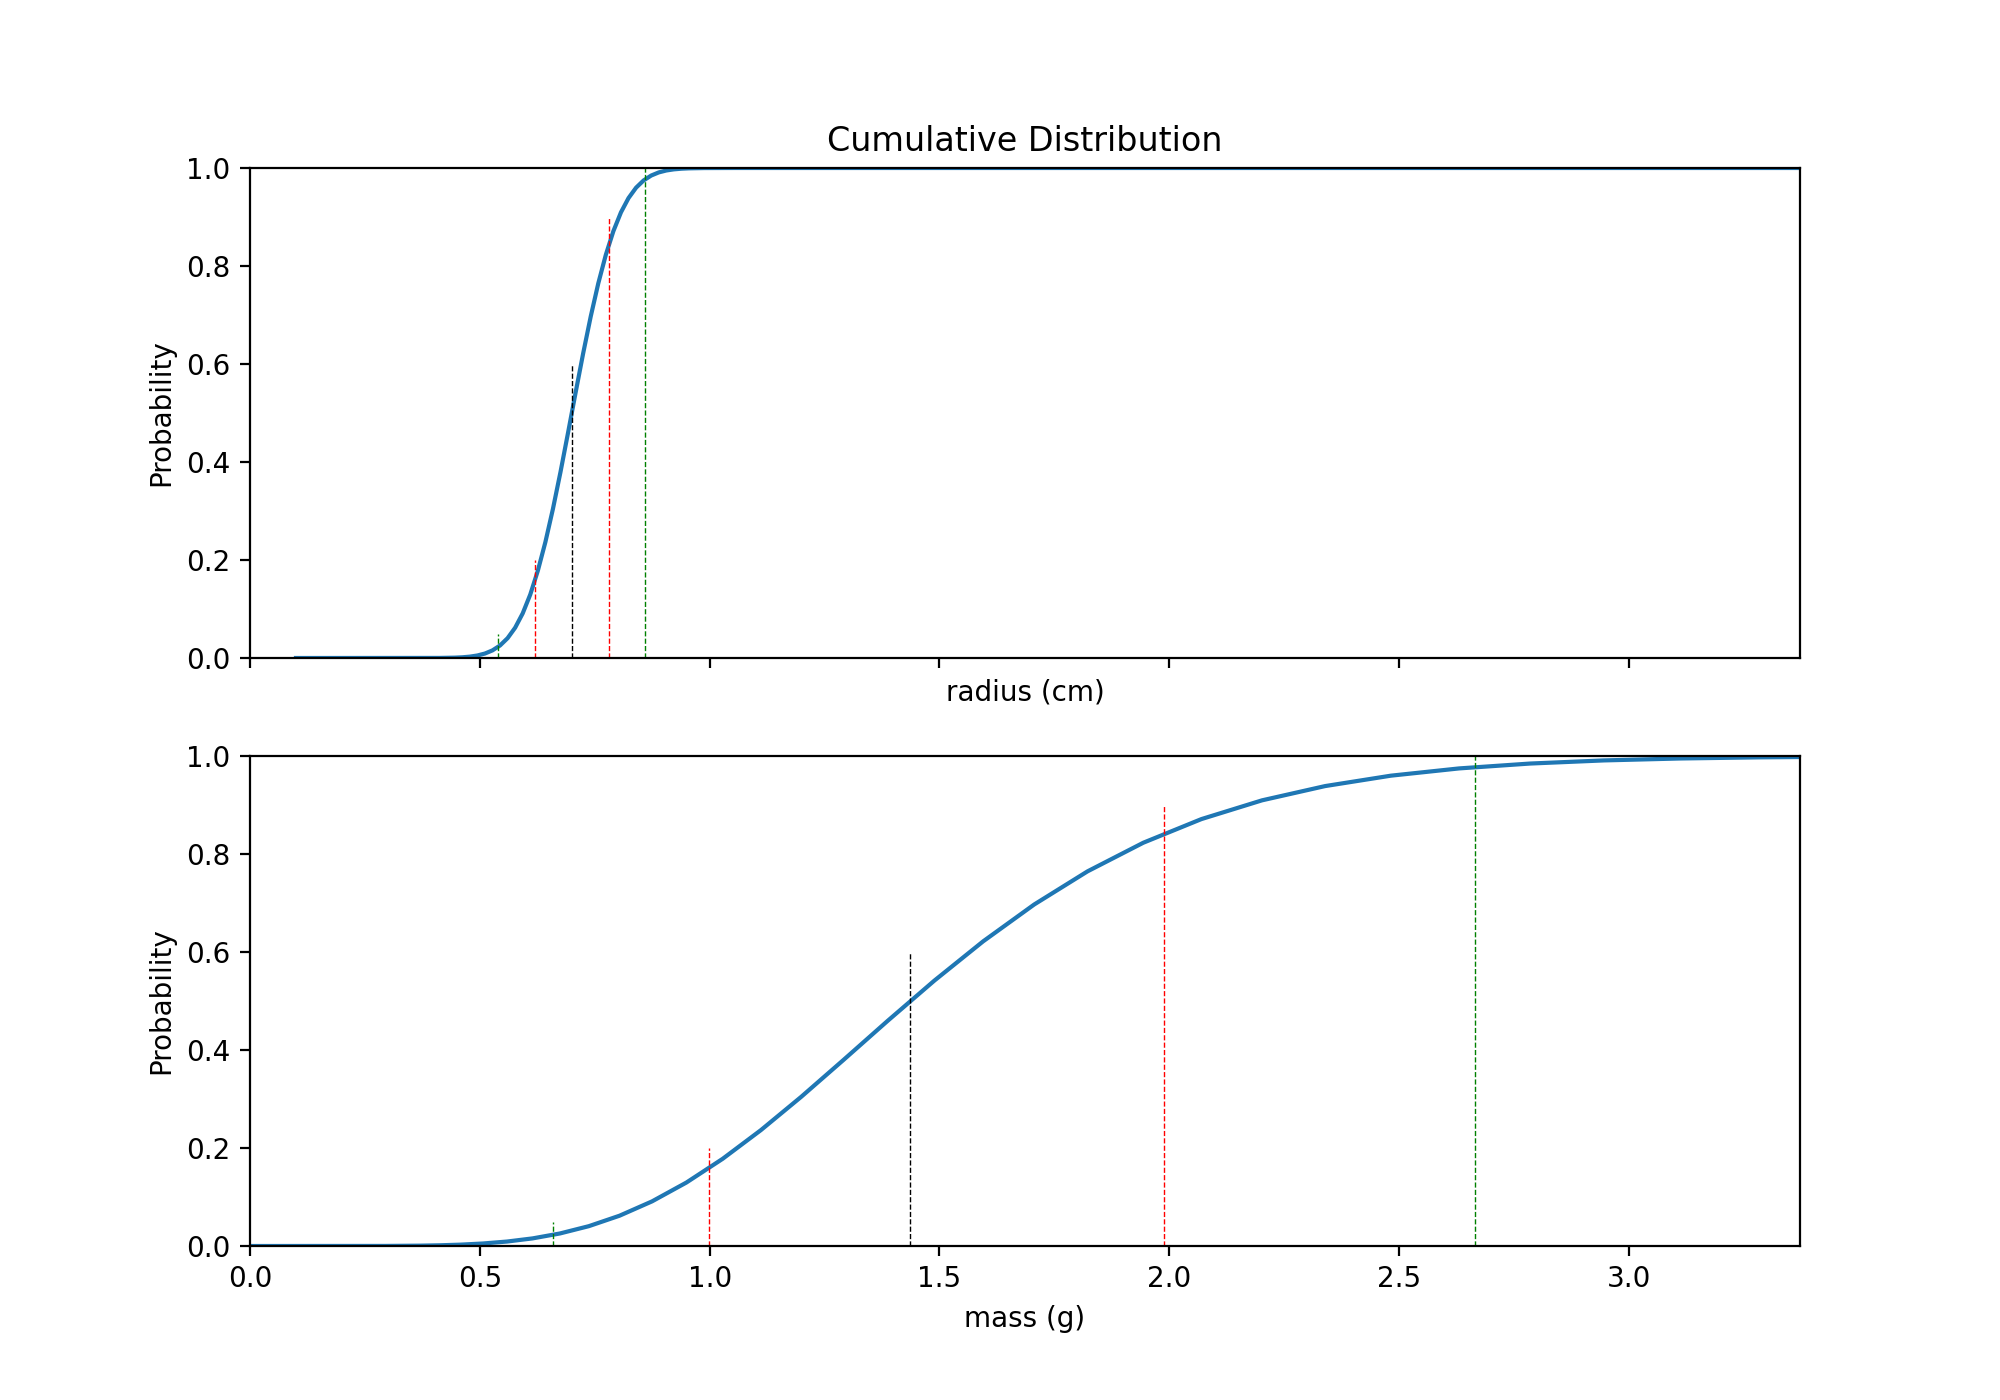
\includegraphics[width=0.8\textwidth]{cdf_after.png}

If $F$ is the original cumulative distribution function, and $g$ is the function that maps the new variable (mass, in this case) to the old one (radius),  then the 
new cumulative distribution function $H$ is given by 

$$H(m) = F(g(m))$$

In this case,   $F$ is the cumulative function for the normal distribution with mean $0.7$ and standard deviation of $0.08$.  $g$ maps the mass to the radius:

$$g(m) =\left(\sqrt[3]{\frac{3}{4 \pi}}\right) x^{\frac{1}{3}}$$

\section{Making a Probability Density Function}

Now we know how to calculate a new cumulative distribution function using the new variable.  However,  we usually want a probability density.

Here is the CDF and the PDF of the mass of the ice spheres:

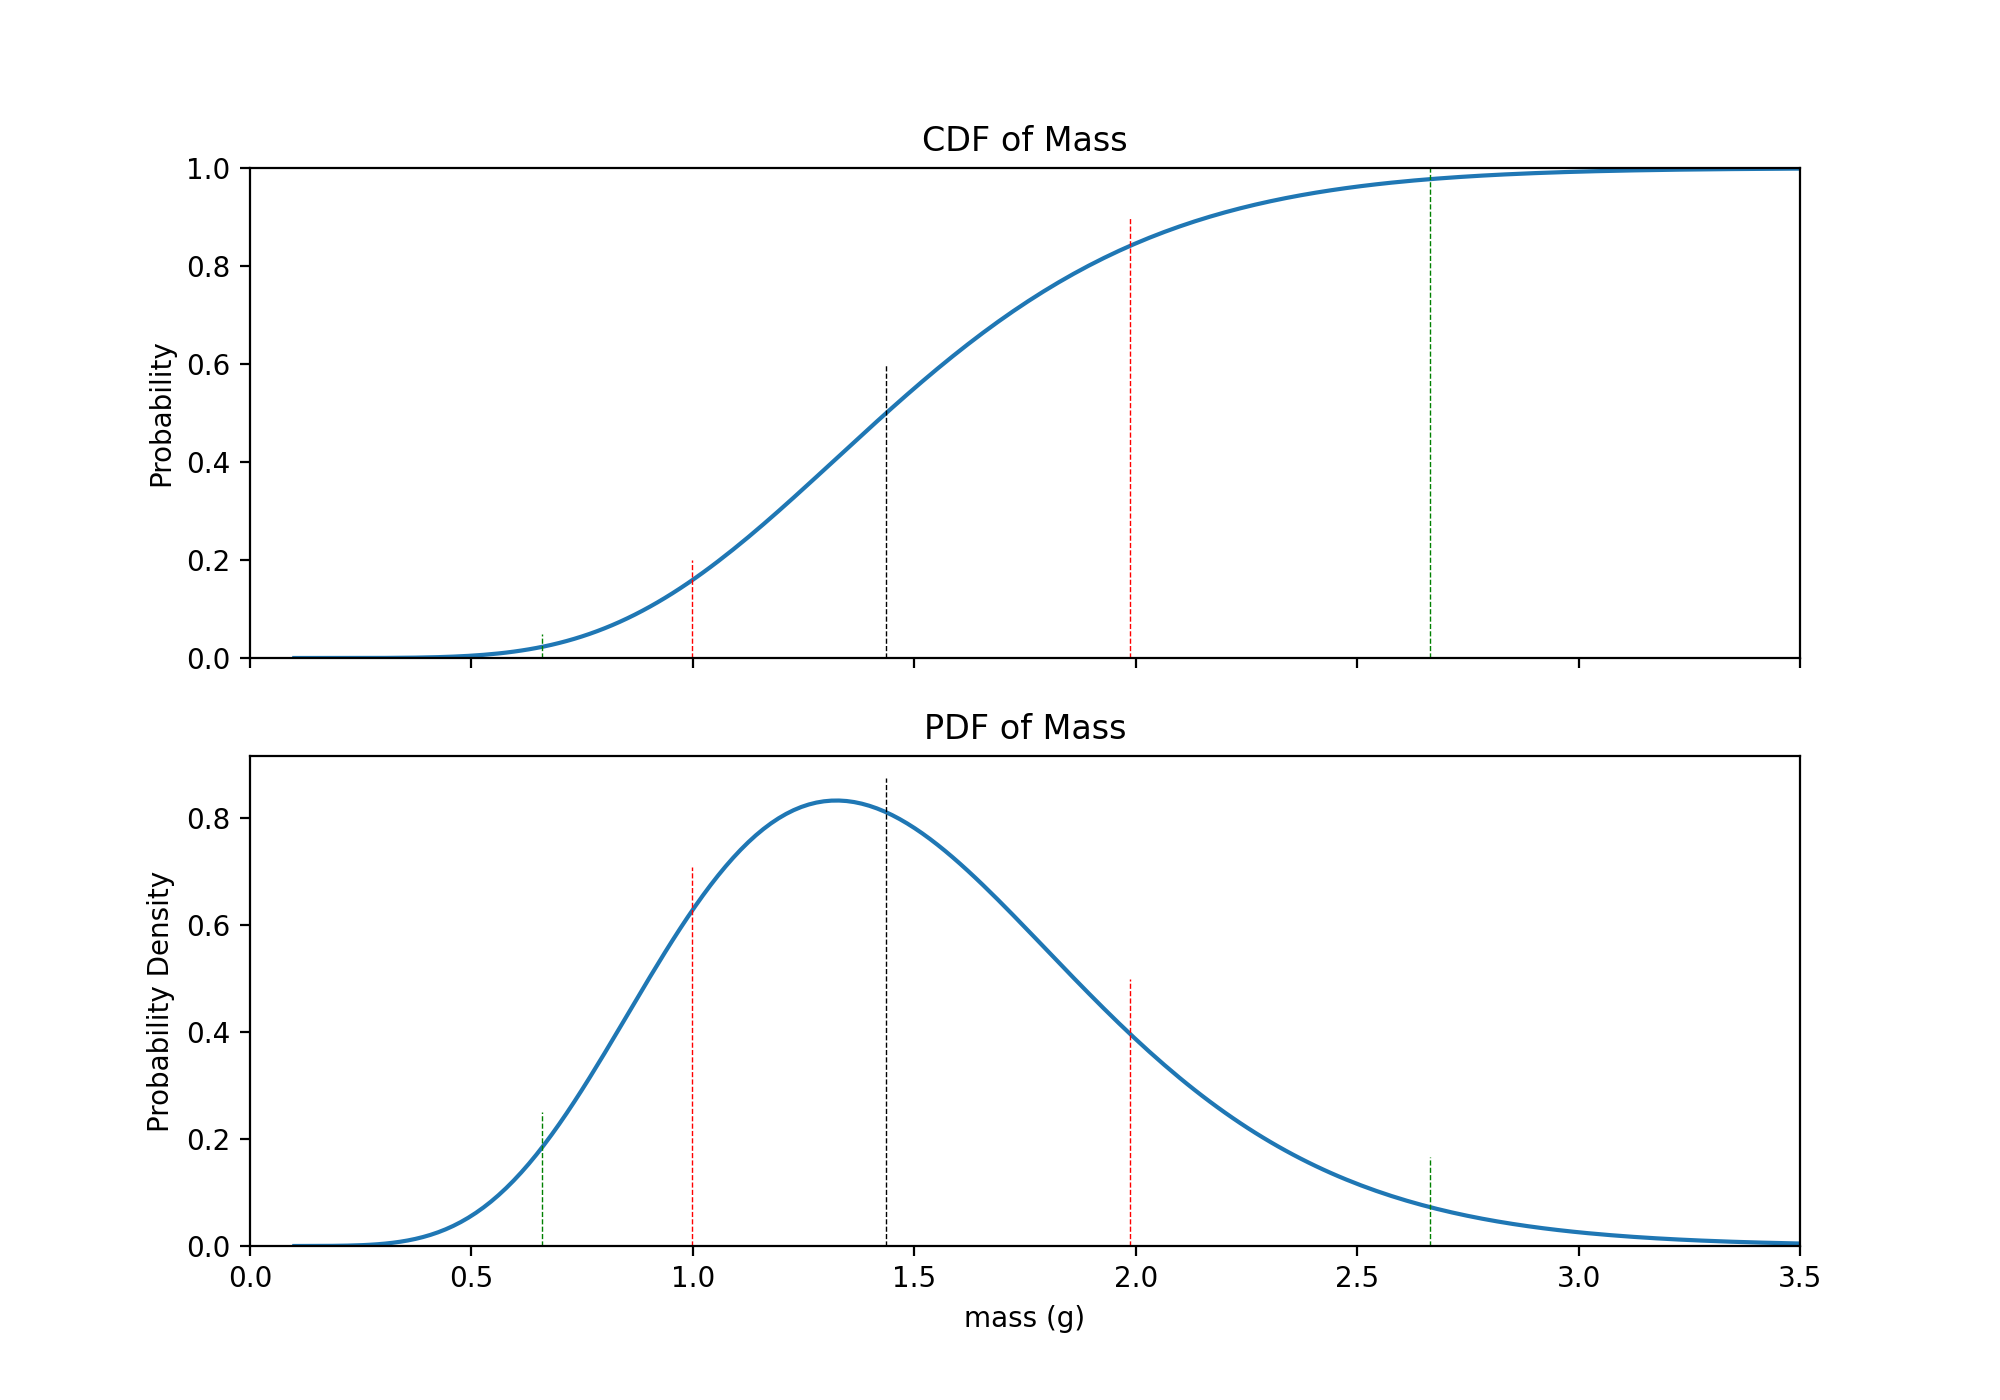
\includegraphics[width=0.8\textwidth]{pdf.png}

Reminder: The probability density function is the derivative of the cumulative distribution function.    We know the CDF is

$$H(m) = F(g(m))$$

By the chain rule:

$$H'(m) = F'(g(m))g'(m)$$

The function $F$ is the cumulative distribution for the normal distribution with mean $0.7$ and standard deviation of $0.08$.  So we know its derivative:

$$F'(x) = \frac{1}{\sigma\sqrt{2\pi}} e^{-\frac{1}{2}\left(\frac{x - \mu}{\sigma}\right)^2}$$

Where  $\mu = 0.7$ and $\sigma = 0.08$.

We've already said that 

$$g(m) = \left(\sqrt[3]{\frac{3}{4 \pi}}\right) m^{\frac{1}{3}}$$

Which is easy to differentiate:

$$g'(m) = \left(\frac{1}{3} \right) \left(\sqrt[3]{\frac{3}{4 \pi}}\right) m^{-\frac{2}{3}}$$

Here, then, is the code to generate that last plot:

\begin{verbatim}
import numpy as np
from scipy.stats import norm
import matplotlib.pyplot as plt

# Constants
MEAN_RADIUS = 0.7
STD_RADIUS = 0.08

# Range to plot
MIN_MASS = 0.1
MAX_MASS = 3.5

# Number of points to plot
N = 200

# Needed for radius_for_mass and d_radius_for_mass
C = np.power(3 / (4 * np.pi), 1/3)

# In these three functions, x can
# be a number or a numpy array

def mass_for_radius(x):
    return 4 * np.pi * np.power(x, 3) / 3

def radius_for_mass(x):
    return C * np.power(x, 1/3)

# Derivative of radius_for_mass()
def d_radius_for_mass(x):
    return (C/3) * np.power(x,-2/3)

# Compute mean and 2 standard deviations in each direction
m_mean = mass_for_radius(MEAN_RADIUS)
m_minus_std = mass_for_radius(MEAN_RADIUS - STD_RADIUS)
m_plus_std = mass_for_radius(MEAN_RADIUS + STD_RADIUS)
m_minus_2std = mass_for_radius(MEAN_RADIUS - 2 * STD_RADIUS)
m_plus_2std = mass_for_radius(MEAN_RADIUS + 2 * STD_RADIUS)

# Make N possible values for mass
m_values = np.linspace(MIN_MASS, MAX_MASS, N)

# Compute g(m) for each of these masses
# That is: What is the radius for each of these masses?
r_values = radius_for_mass(m_values)

# Compute F(g(m)) for each of these masses
# That is: What is the cumulative distribution for each those radii?
cdf_values = norm.cdf(r_values, loc=MEAN_RADIUS, scale=STD_RADIUS)

# Compute g'(m) for each of these masses
dg_values = d_radius_for_mass(m_values)

# What is F'(g(m))g'(m)?
pdf_values = norm.pdf(r_values, loc=MEAN_RADIUS, scale=STD_RADIUS) * dg_values

# Sanity check: It should integrate to a little less then 1.0
dx = (MAX_MASS - MIN_MASS)/N
area_under_curve = pdf_values.sum() * dx
print(f"Integral from {MIN_MASS:.2f} to {MAX_MASS:.2f}: {area_under_curve:.3f}")

# Make a figure with two axes
fig, axs = plt.subplots(nrows=2, sharex=True, figsize=(10, 7), dpi=200)

# Draw the CDF on the second axix
axs[0].set_title("CDF of Mass")
axs[0].set_ylim(bottom=0.0, top=1.0)
axs[0].set_xlim(left=0.0, right=MAX_MASS)
axs[0].set_ylabel("Probability")
axs[0].plot(m_values, cdf_values)

# Add lines for mean,  mean-std, and mean+std
axs[0].vlines(m_minus_2std, 0, 0.05, "g", linestyle="dashed",lw=0.5)
axs[0].vlines(m_minus_std, 0, 0.2, "r", linestyle="dashed",lw=0.5)
axs[0].vlines(m_mean, 0, 0.6, "k", linestyle="dashed",lw=0.5)
axs[0].vlines(m_plus_std, 0, 0.9, "r", linestyle="dashed",lw=0.5)
axs[0].vlines(m_plus_2std, 0, 1.0, "g", linestyle="dashed",lw=0.5)

# How high does the pdf go?
max_density = pdf_values.max()

# Draw the PDF on the second axix
axs[1].set_title("PDF of Mass")
axs[1].set_ylim(bottom=0.0, top=max_density * 1.1)
axs[1].set_xlim(left=0.0, right=MAX_MASS)
axs[1].set_xlabel("mass (g)")
axs[1].set_ylabel("Probability Density")
axs[1].plot(m_values, pdf_values)

# Add lines for mean,  mean-std, and mean+std
axs[1].vlines(m_minus_2std, 0, max_density * .3, "g", linestyle="dashed",lw=0.5)
axs[1].vlines(m_minus_std, 0, max_density * .85 , "r", linestyle="dashed",lw=0.5)
axs[1].vlines(m_mean, 0, max_density * 1.05, "k", linestyle="dashed",lw=0.5)
axs[1].vlines(m_plus_std, 0, max_density * .6, "r", linestyle="dashed",lw=0.5)
axs[1].vlines(m_plus_2std, 0, max_density * .2, "g", linestyle="dashed",lw=0.5)
fig.savefig("pdf.png")
\end{verbatim}

\section{Decreasing Conversions}

The last case (mass and radius) is pretty straightforward because the function $g$ is always increasing.  What if we have a change of variables where 
$g$ is decreasing.   For example,  $V= IR$ so $\frac{V}{R} = I$.

Let's say that you work at a lightbulb factory and you sample the lightbulbs to see what their resistance is.  You find the resistances of the lightbulbs are normally distributed with a mean of 24 ohms and a standard deviation of 3 ohms.  The voltage will be exactly 12 volts.  What is the PDF of the currents that will pass through the lightbulbs?

$$I = \frac{12}{R}$$

so 

$$g(x) = \frac{12}{x}$$

is the function that will convert the current to resistance.  Taking the derivative,  we get:

$$g'(i) = -\frac{12}{x^2}$$










